% Practice Test 23 — Indiana Edition
% Questions: 30 (15 MC + 15 SA)
% Generated by scripts/generate_practice_tests.py

\begin{practiceQuestion}{1-3-q05}{mc}
\begin{questionText}
A car travels at a constant speed. It goes $150$ miles in $2.5$ hours. What is the constant of proportionality?
\end{questionText}
\choiceA{$30$ mph}
\choiceB{$60$ mph}
\choiceC{$75$ mph}
\choiceD{$150$ mph}
\correctAnswer{B}
\explanation{$k = \frac{150}{2.5} = 60$ miles per hour.}
\end{practiceQuestion}

\begin{practiceQuestion}{1-5-q30}{gsa}
\begin{questionText}
Two friends start walking at the same time. The graph shows their distances. How many miles apart are they after $6$ hours?

\begin{center}
\begin{tikzpicture}[scale=0.7]
  \draw[step=1,gray!20,thin] (0,0) grid (7,8);
  \draw[thick,->] (0,0) -- (7.5,0) node[right]{\small Hours};
  \draw[thick,->] (0,0) -- (0,8.5) node[above]{\small Miles};
  \foreach \x in {1,...,7} \draw (\x,0.07) -- (\x,-0.07) node[below]{\tiny \x};
  \foreach \y in {1,...,8} \draw (0.07,\y) -- (-0.07,\y) node[left]{\tiny \y};
  \draw[thick,funBlue] (0,0) -- (6,7.2);
  \fill[funBlue] (0,0) circle (2pt);
  \fill[funBlue] (5,6) circle (2.5pt) node[above left]{\small $(5, 6)$};
  \node[above,funBlue] at (5.5,6.6) {\small Ava};
  \draw[thick,funRed] (0,0) -- (6,4.8);
  \fill[funRed] (0,0) circle (2pt);
  \fill[funRed] (5,4) circle (2.5pt) node[below right]{\small $(5, 4)$};
  \node[below right,funRed] at (5.5,4.4) {\small Ben};
\end{tikzpicture}
\end{center}
\end{questionText}
\correctAnswer{$2.4$ miles}
\explanation{Ava: $k = \frac{6}{5} = 1.2$ mph; at $6$ hr: $1.2 \times 6 = 7.2$ mi. Ben: $k = \frac{4}{5} = 0.8$ mph; at $6$ hr: $0.8 \times 6 = 4.8$ mi. Difference: $7.2 - 4.8 = 2.4$ miles.}
\end{practiceQuestion}

\begin{practiceQuestion}{1-6-q21}{sa}
\begin{questionText}
A scale drawing uses $1$ cm $= 4.5$ m. If a building is $27$ m tall, how tall is it in the drawing?
\end{questionText}
\correctAnswer{$6$ cm}
\explanation{$\frac{1}{4.5} = \frac{x}{27}$. Cross-multiply: $4.5x = 27$, so $x = 6$ cm.}
\end{practiceQuestion}

\begin{practiceQuestion}{2-2-q14}{mc}
\begin{questionText}
$27$ out of $180$ students earned an A on the exam. What percent earned an A?
\end{questionText}
\choiceA{$12\%$}
\choiceB{$15\%$}
\choiceC{$18\%$}
\choiceD{$27\%$}
\correctAnswer{B}
\explanation{$\frac{27}{180} = \frac{p}{100}$. Cross-multiply: $180p = 2700$. Divide: $p = 15\%$.}
\end{practiceQuestion}

\begin{practiceQuestion}{2-5-q22}{sa}
\begin{questionText}
Estimate a $20\%$ tip on a $\$93$ bill. Round the bill first, then calculate.
\end{questionText}
\correctAnswer{About $\$18.60$}
\explanation{Round to $\$93$. Find $10\%$: $\$9.30$. Double for $20\%$: $9.30 \times 2 = \$18.60$.}
\end{practiceQuestion}

\begin{practiceQuestion}{2-7-q28}{gmc}
\begin{questionText}
The number line below shows an estimated value and an actual value. What is the percent error?

\begin{center}
\begin{tikzpicture}[scale=0.6]
  \draw[thick,->] (-0.5,0) -- (11,0);
  \foreach \x/\lab in {0/0,2/10,4/20,6/30,8/40,10/50} {
    \draw (\x,0.15) -- (\x,-0.15) node[below,font=\small] {\lab};
  }
  % Actual at 40
  \filldraw[funGreen] (8,0) circle (4pt);
  \node[above,font=\small,funGreen!80!black] at (8,0.3) {Actual: $40$};
  % Estimated at 35
  \filldraw[funRed] (7,0) circle (4pt);
  \node[below=10pt,font=\small,funRed] at (7,-0.15) {Estimated: $35$};
  % Arrow showing difference
  \draw[thick,<->,funOrange] (7,0.7) -- (8,0.7) node[midway,above,font=\small]{$5$};
\end{tikzpicture}
\end{center}
\end{questionText}
\choiceA{$5\%$}
\choiceB{$10\%$}
\choiceC{$12.5\%$}
\choiceD{$14.3\%$}
\correctAnswer{C}
\explanation{$\frac{|35-40|}{40} \times 100 = \frac{5}{40} \times 100 = 12.5\%$.}
\end{practiceQuestion}

\begin{practiceQuestion}{3-1-q15}{mc}
\begin{questionText}
An elevator goes $3$ floors up from the lobby, then $7$ floors down. Which integer describes its final position relative to the lobby?
\end{questionText}
\choiceA{$4$}
\choiceB{$-4$}
\choiceC{$10$}
\choiceD{$-10$}
\correctAnswer{B}
\explanation{Up $3$ floors, then down $7$: $3 + (-7) = -4$. The elevator is $4$ floors below the lobby.}
\end{practiceQuestion}

\begin{practiceQuestion}{3-2-q13}{mc}
\begin{questionText}
A bank account has $-\$50$ (overdrawn). A deposit of $\$75$ is made. What is the new balance?
\end{questionText}
\choiceA{$-\$125$}
\choiceB{$-\$25$}
\choiceC{$\$25$}
\choiceD{$\$125$}
\correctAnswer{C}
\explanation{$(-50) + 75 = 25$. The deposit is larger than the overdraft, so the balance becomes positive.}
\end{practiceQuestion}

\begin{practiceQuestion}{4-2-q08}{mc}
\begin{questionText}
Simplify $\frac{1}{3}x + \frac{2}{3}x$.


\begin{center}
\fractionBar{1}{3}
\hspace{1cm}
\fractionBar{2}{3}
\end{center}
\end{questionText}
\choiceA{$\frac{2}{9}x$}
\choiceB{$x$}
\choiceC{$\frac{3}{6}x$}
\choiceD{$\frac{1}{3}x^2$}
\correctAnswer{B}
\explanation{The coefficients are $\frac{1}{3}$ and $\frac{2}{3}$. Add: $\frac{1}{3} + \frac{2}{3} = \frac{3}{3} = 1$. Result: $1x = x$.}
\end{practiceQuestion}

\begin{practiceQuestion}{4-3-q25}{sa}
\begin{questionText}
Expand and simplify $-4(a - 2) + 3(a + 5) - 7$.
\end{questionText}
\correctAnswer{$-a + 16$}
\explanation{Expand: $-4a + 8 + 3a + 15 - 7$. Combine: $(-4a + 3a) + (8 + 15 - 7) = -a + 16$.}
\end{practiceQuestion}

\begin{practiceQuestion}{5-4-q27}{gmc}
\begin{questionText}
Use the fraction bar model to solve: $\dfrac{2}{3}x = 8$. What is $x$?

\begin{center}
\begin{tikzpicture}[scale=0.6]
  % Full bar = x
  \draw[thick,fill=funBlue!15] (0,2) rectangle (12,3);
  \node at (6,2.5) {$x$};
  % 2/3 of bar highlighted
  \draw[thick,fill=funOrange!30] (0,0) rectangle (8,1);
  \node at (4,0.5) {$\frac{2}{3}x = 8$};
  \draw[thick,fill=gray!15] (8,0) rectangle (12,1);
  \node at (10,0.5) {$?$};
  % Dividers
  \draw[dashed] (4,0) -- (4,1);
  \draw[dashed] (4,2) -- (4,3);
  \draw[dashed] (8,0) -- (8,3);
  \node[below] at (2,-0.2) {$\frac{1}{3}$};
  \node[below] at (6,-0.2) {$\frac{1}{3}$};
  \node[below] at (10,-0.2) {$\frac{1}{3}$};
\end{tikzpicture}
\end{center}
\end{questionText}
\choiceA{$x = 12$}
\choiceB{$x = 16$}
\choiceC{$x = 10$}
\choiceD{$x = 5\dfrac{1}{3}$}
\correctAnswer{A}
\explanation{If $\frac{2}{3}x = 8$, then each $\frac{1}{3}$ of $x$ is $4$. So $x = 3 \times 4 = 12$.}
\end{practiceQuestion}

\begin{practiceQuestion}{5-5-q10}{mc}
\begin{questionText}
Solve $3x + 7 \leq 25$.
\end{questionText}
\choiceA{$x \leq \dfrac{32}{3}$}
\choiceB{$x \leq 6$}
\choiceC{$x \geq 6$}
\choiceD{$x \leq 9$}
\correctAnswer{B}
\explanation{Subtract $7$: $3x \leq 18$. Divide by $3$: $x \leq 6$.}
\end{practiceQuestion}

\begin{practiceQuestion}{5-6-q24}{sa}
\begin{questionText}
What inequality is shown by a closed circle at $-6$ with shading to the right?
\end{questionText}
\correctAnswer{$x \geq -6$}
\explanation{Closed circle means $-6$ is included, shading right means values greater than or equal to $-6$: $x \geq -6$.}
\end{practiceQuestion}

\begin{practiceQuestion}{6-1-q30}{gsa}
\begin{questionText}
A scale drawing of a soccer field is shown on the grid below. Each grid square represents $10$ m $\times$ $10$ m in real life. What is the actual perimeter of the field?

\begin{center}
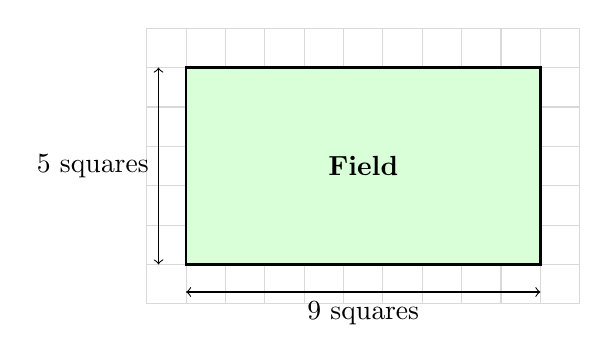
\begin{tikzpicture}[scale=0.5]
  \draw[step=1,gray!30,thin] (0,0) grid (11,7);
  \draw[thick,fill=green!15] (1,1) rectangle (10,6);
  \node at (5.5,3.5) {\textbf{Field}};
  \draw[<->] (1,0.3) -- (10,0.3);
  \node[below] at (5.5,0.3) {$9$ squares};
  \draw[<->] (0.3,1) -- (0.3,6);
  \node[left] at (0.3,3.5) {$5$ squares};
\end{tikzpicture}
\end{center}
\end{questionText}
\correctAnswer{$280$ m}
\explanation{Each square is $10$ m. Length: $9 \times 10 = 90$ m. Width: $5 \times 10 = 50$ m. Perimeter: $2(90 + 50) = 2(140) = 280$ m.}
\end{practiceQuestion}

\begin{practiceQuestion}{6-3-q22}{sa}
\begin{questionText}
Two sides of a triangle are $5$ cm and $5$ cm with an included angle of $60°$. What type of triangle is formed?
\end{questionText}
\correctAnswer{Equilateral triangle}
\explanation{Two equal sides with a $60°$ included angle gives a triangle where all angles are $60°$ (isosceles with $60°$ forces equilateral). All three sides are $5$ cm.}
\end{practiceQuestion}

\begin{practiceQuestion}{6-4-q25}{sa}
\begin{questionText}
A triangle has angles $60°$, $60°$, and $60°$, and one side measures $10$ cm. How many triangles can be drawn?
\end{questionText}
\correctAnswer{Exactly one}
\explanation{AAA alone gives many, but specifying a side length fixes the size. A triangle with all $60°$ angles is equilateral, so all sides are $10$ cm. Exactly one triangle.}
\end{practiceQuestion}

\begin{practiceQuestion}{6-5-q21}{sa}
\begin{questionText}
What shape is the cross-section when a cone is sliced vertically through its apex?
\end{questionText}
\correctAnswer{A triangle}
\explanation{A vertical slice through the apex of a cone produces an isosceles triangle. The base of the triangle is a diameter of the cone's base.}
\end{practiceQuestion}

\begin{practiceQuestion}{6-6-q11}{mc}
\begin{questionText}
Which statement about vertical angles is always true?
\end{questionText}
\choiceA{They are supplementary}
\choiceB{They are complementary}
\choiceC{They are equal}
\choiceD{They sum to $360°$}
\correctAnswer{C}
\explanation{Vertical angles are always equal. They are formed by two intersecting lines, and the opposite angles are congruent.}
\end{practiceQuestion}

\begin{practiceQuestion}{6-7-q22}{sa}
\begin{questionText}
A triangle has vertices $A(2, 1)$, $B(6, 1)$, and $C(6, 4)$. Reflect the triangle over the $y$-axis. List the new vertices.
\end{questionText}
\correctAnswer{$A'(-2, 1)$, $B'(-6, 1)$, $C'(-6, 4)$}
\explanation{Over the $y$-axis: negate $x$, keep $y$. $(2,1) \to (-2,1)$, $(6,1) \to (-6,1)$, $(6,4) \to (-6,4)$.}
\end{practiceQuestion}

\begin{practiceQuestion}{7-3-q28}{gmc}
\begin{questionText}
A square has a circle inscribed inside it as shown. The side of the square is $10$ cm. What is the area of the circle? Use $\pi \approx 3.14$.

\begin{center}
\begin{tikzpicture}[scale=0.4]
  \draw[thick] (-5,-5) rectangle (5,5);
  \draw[thick,funBlue,fill=funBlue!10] (0,0) circle (5);
  \draw[thick,funRed,<->] (-5,-6) -- (5,-6);
  \node[below,funRed] at (0,-6) {$10$ cm};
  \fill (0,0) circle (2pt);
\end{tikzpicture}
\end{center}
\end{questionText}
\choiceA{$31.4$ cm$^2$}
\choiceB{$78.5$ cm$^2$}
\choiceC{$100$ cm$^2$}
\choiceD{$314$ cm$^2$}
\correctAnswer{B}
\explanation{The circle's diameter equals the side of the square: $d = 10$, so $r = 5$ cm. $A = \pi r^2 = 3.14 \times 25 = 78.5$ cm$^2$.}
\end{practiceQuestion}

\begin{practiceQuestion}{7-4-q23}{sa}
\begin{questionText}
A rectangular patio is $12$ ft by $8$ ft. A circular hot tub with a diameter of $6$ ft is placed on the patio. What is the area of the patio NOT covered by the hot tub? Use $\pi \approx 3.14$.
\end{questionText}
\correctAnswer{$67.74$ ft$^2$}
\explanation{Patio: $12 \times 8 = 96$ ft$^2$. Hot tub: $\pi r^2 = 3.14 \times 9 = 28.26$ ft$^2$. Remaining: $96 - 28.26 = 67.74$ ft$^2$.}
\end{practiceQuestion}

\begin{practiceQuestion}{7-5-q02}{mc}
\begin{questionText}
What is the surface area of a rectangular prism with length $5$ cm, width $3$ cm, and height $2$ cm?
\end{questionText}
\choiceA{$30$ cm$^2$}
\choiceB{$62$ cm$^2$}
\choiceC{$46$ cm$^2$}
\choiceD{$31$ cm$^2$}
\correctAnswer{B}
\explanation{$SA = 2(5 \times 3) + 2(5 \times 2) + 2(3 \times 2) = 30 + 20 + 12 = 62$ cm$^2$.}
\end{practiceQuestion}

\begin{practiceQuestion}{7-6-q03}{mc}
\begin{questionText}
What is the volume of a cube with side length $5$ m?
\end{questionText}
\choiceA{$15$ m$^3$}
\choiceB{$25$ m$^3$}
\choiceC{$125$ m$^3$}
\choiceD{$150$ m$^3$}
\correctAnswer{C}
\explanation{$V = s^3 = 5^3 = 125$ m$^3$.}
\end{practiceQuestion}

\begin{practiceQuestion}{8-1-q21}{sa}
\begin{questionText}
A random sample of $50$ apples from an orchard found that $6$ were bruised. If the orchard has $3{,}000$ apples, about how many are bruised?
\end{questionText}
\correctAnswer{$360$}
\explanation{$\frac{6}{50} = 12\%$. Then $12\%$ of $3{,}000 = 360$.}
\end{practiceQuestion}

\begin{practiceQuestion}{8-3-q22}{sa}
\begin{questionText}
Team A: mean $60$, MAD $4$. Team B: mean $70$, MAD $3$. Is the difference in means meaningful? Explain briefly.
\end{questionText}
\correctAnswer{Yes; the means are about $2.5$ to $3.3$ MADs apart}
\explanation{Difference $= 10$. Using MAD of $4$: $\frac{10}{4} = 2.5$. Using MAD of $3$: $\frac{10}{3} \approx 3.3$. Both are greater than $2$, so the difference is meaningful.}
\end{practiceQuestion}

\begin{practiceQuestion}{8-4-q05}{mc}
\begin{questionText}
Data set: $20, 22, 25, 27, 30, 32, 35$. What is the IQR?
\end{questionText}
\choiceA{$15$}
\choiceB{$10$}
\choiceC{$7$}
\choiceD{$5$}
\correctAnswer{B}
\explanation{$Q_1 = 22$, $Q_3 = 32$. IQR $= 32 - 22 = 10$.}
\end{practiceQuestion}

\begin{practiceQuestion}{8-7-q22}{sa}
\begin{questionText}
A line graph shows temperatures: Mon $72°$, Tue $68°$, Wed $70°$, Thu $75°$, Fri $73°$. What is the range of temperatures?
\end{questionText}
\correctAnswer{$7°$}
\explanation{Range $= 75 - 68 = 7°$.}
\end{practiceQuestion}

\begin{practiceQuestion}{9-4-q11}{mc}
\begin{questionText}
A bag contains $5$ yellow and $5$ purple marbles. Lisa picks a marble, records the color, and replaces it $40$ times. She gets yellow $24$ times. Which statement is correct?
\end{questionText}
\choiceA{The model predicts $P(\text{yellow}) = 0.5$, and the experiment gives $P(\text{yellow}) = 0.6$, so there is a small difference}
\choiceB{The model is wrong because $24 \neq 20$}
\choiceC{The model predicts $P(\text{yellow}) = 0.6$}
\choiceD{The experiment proves yellow is more likely than purple}
\correctAnswer{A}
\explanation{Predicted: $\frac{5}{10} = 0.5$. Experimental: $\frac{24}{40} = 0.6$. The small difference is expected from natural variation.}
\end{practiceQuestion}

\begin{practiceQuestion}{9-6-q20}{sa}
\begin{questionText}
A coin is flipped and a die is rolled. What is the probability of getting tails and a $1$? Write your answer as a fraction.
\end{questionText}
\correctAnswer{$\frac{1}{12}$}
\explanation{$P(\text{tails}) = \frac{1}{2}$, $P(1) = \frac{1}{6}$. $P = \frac{1}{2} \times \frac{1}{6} = \frac{1}{12}$.}
\end{practiceQuestion}

\begin{practiceQuestion}{9-7-q12}{mc}
\begin{questionText}
How does increasing the number of trials in a simulation affect the results?
\end{questionText}
\choiceA{The results become less reliable}
\choiceB{The experimental probability gets closer to the theoretical probability}
\choiceC{The results stay exactly the same}
\choiceD{The simulation takes less time}
\correctAnswer{B}
\explanation{More trials produce more reliable estimates. The experimental probability approaches the theoretical value as trials increase.}
\end{practiceQuestion}
